\begin{frame}{目录}
    \tableofcontents
\end{frame}

\section{基本概念}

\begin{frame}{网格世界}
    \begin{center}
        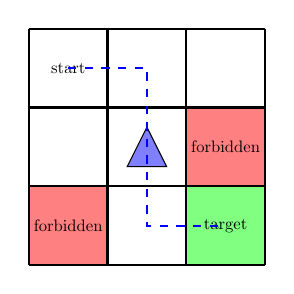
\begin{tikzpicture}
            % 填充指定格子为红色
            \fill[red!50] (2,1) rectangle (3,2); % 第2行第3列 (索引 (2,1))
            \fill[red!50] (0,0) rectangle (1,1); % 第3行第1列 (索引 (0,0))
            \fill[green!50] (2,0) rectangle (3,1); % 第3行第1列 (索引 (0,0))

            % 画3x3网格
            \draw[thick] (0,0) grid (3,3);
            
            % 标记状态编号 (行列索引)
            \foreach \x in {0,1,2} {
                \foreach \y in {0,1,2} {
                    \node at (\x+0.5, 2.5-\y){};
                }
            }
            % 在 (0,2) 位置放一个小三角形,代表 agent
            \draw[fill=blue!50] (1.25,1.25) -- (1.75,1.25) -- (1.5,1.75) -- cycle;

            \node[scale=0.6] at (0.5, 2.5) {start};

            % 在红色格子内写 "forbidden"
            \node[scale=0.6] at (2.5, 1.5) {forbidden};
            \node[scale=0.6] at (0.5, 0.5) {forbidden};

            % 在绿色格子内写 "target"
            \node[scale=0.6] at (2.5, 0.5) {target};

            \draw[dashed, thick, color=blue] (0.5,2.5) -- (1.5,2.5) -- (1.5,0.5) -- (2.5,0.5);
        \end{tikzpicture}
    \end{center}
    \begin{itemize}
        \item 格子:可通过/禁止通过/目标,边界
    \end{itemize}
    任务:
    \begin{itemize}
        \item 给定一个起始点,找出一条“好”的路径到终点。
        \item 怎么定义“好”:尽量避免forbidden的格子,少走重复的路,尽量不要撞到边界。
    \end{itemize}
\end{frame}
%------------------------------------------------

\begin{frame}{状态}
    \textbf{状态}:智能体在环境中被描述的状态。
    在网格世界中,智能体的位置就是他的状态。网格世界中一共有9个可能的位置,所以智能体也就有9个可能的状态:$s_1, s_2,\cdots, s_9$。
    \begin{center}
        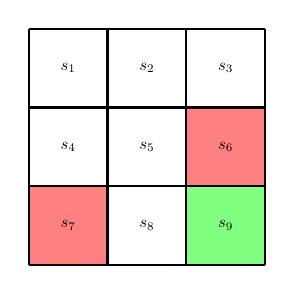
\begin{tikzpicture}
            % 填充指定格子为红色
            \fill[red!50] (2,1) rectangle (3,2); % 第2行第3列 (索引 (2,1))
            \fill[red!50] (0,0) rectangle (1,1); % 第3行第1列 (索引 (0,0))
            \fill[green!50] (2,0) rectangle (3,1); % 第3行第1列 (索引 (0,0))

            % 画3x3网格
            \draw[thick] (0,0) grid (3,3);
            
            % 标记状态编号 (行列索引)
            \foreach \x in {0,1,2} {
                \foreach \y in {0,1,2} {
                    \node at (\x+0.5, 2.5-\y){};
                }
            }

            % 在红色格子内写 "forbidden"
            \node[scale=0.6] at (0.5, 2.5) {$s_1$};
            \node[scale=0.6] at (1.5, 2.5) {$s_2$};
            \node[scale=0.6] at (2.5, 2.5) {$s_3$};
            \node[scale=0.6] at (0.5, 1.5) {$s_4$};
            \node[scale=0.6] at (1.5, 1.5) {$s_5$};
            \node[scale=0.6] at (2.5, 1.5) {$s_6$};
            \node[scale=0.6] at (0.5, 0.5) {$s_7$};
            \node[scale=0.6] at (1.5, 0.5) {$s_8$};
            \node[scale=0.6] at (2.5, 0.5) {$s_9$};

        \end{tikzpicture}
    \end{center}
    \textbf{状态空间}:所有状态的集合$\mathcal{S}=\{s_i\}_{i=1}^9$
\end{frame}

\begin{frame}{动作}
    \textbf{动作}:对于每个状态,有5个可能的动作:$a_1, a_2,\cdots,a_5$
    \begin{itemize}
        \item $a_1$:向上移动
        \item $a_2$:向右移动
        \item $a_3$:向下移动
        \item $a_4$:向左移动
        \item $a_5$:停留
    \end{itemize}
    \begin{center}
        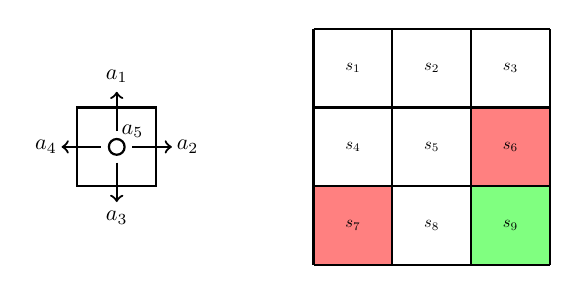
\begin{tikzpicture}
                % 行为格子 (左侧的 1x1 格子)
            \draw[thick] (-3,1) rectangle (-2,2);
            
            % 中心圆圈 (表示Agent停留)
            \draw[thick] (-2.5,1.5) circle (0.1);
            \node[scale=0.8] at (-2.3, 1.7) {$a_5$}; % 标注 a5 (停留)
            
            % 画四个方向的箭头
            \draw[->, thick] (-2.5, 1.7) -- (-2.5, 2.2); % 上
            \node[scale=0.8] at (-2.5, 2.4) {$a_1$};
            \draw[->, thick] (-2.5, 1.3) -- (-2.5, 0.8); % 下
            \node[scale=0.8] at (-2.5, 0.6) {$a_3$};
            \draw[->, thick] (-2.3, 1.5) -- (-1.8, 1.5);  % 右
            \node[scale=0.8] at (-1.6, 1.5) {$a_2$};
            \draw[->, thick] (-2.7, 1.5) -- (-3.2, 1.5); % 左
            \node[scale=0.8] at (-3.4, 1.5) {$a_4$};
            % 填充指定格子为红色
            \fill[red!50] (2,1) rectangle (3,2); % 第2行第3列 (索引 (2,1))
            \fill[red!50] (0,0) rectangle (1,1); % 第3行第1列 (索引 (0,0))
            \fill[green!50] (2,0) rectangle (3,1); % 第3行第1列 (索引 (0,0))

            % 画3x3网格
            \draw[thick] (0,0) grid (3,3);
            
            % 标记状态编号 (行列索引)
            \foreach \x in {0,1,2} {
                \foreach \y in {0,1,2} {
                    \node at (\x+0.5, 2.5-\y){};
                }
            }

            % 在红色格子内写 "forbidden"
            \node[scale=0.6] at (0.5, 2.5) {$s_1$};
            \node[scale=0.6] at (1.5, 2.5) {$s_2$};
            \node[scale=0.6] at (2.5, 2.5) {$s_3$};
            \node[scale=0.6] at (0.5, 1.5) {$s_4$};
            \node[scale=0.6] at (1.5, 1.5) {$s_5$};
            \node[scale=0.6] at (2.5, 1.5) {$s_6$};
            \node[scale=0.6] at (0.5, 0.5) {$s_7$};
            \node[scale=0.6] at (1.5, 0.5) {$s_8$};
            \node[scale=0.6] at (2.5, 0.5) {$s_9$};

        \end{tikzpicture}
    \end{center}
    \textbf{状态的动作空间}:智能体在一个状态可以做的所有动作的集合。$\mathcal{A}(s_i)=\{a_k\}_{k=1}^5$

    \textbf{问题}:不同状态的动作空间一样吗?
\end{frame}

\begin{frame}{状态转移}
    \begin{center}
        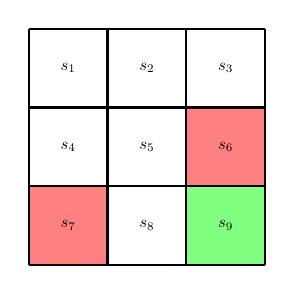
\begin{tikzpicture}
            % 填充指定格子为红色
            \fill[red!50] (2,1) rectangle (3,2); % 第2行第3列 (索引 (2,1))
            \fill[red!50] (0,0) rectangle (1,1); % 第3行第1列 (索引 (0,0))
            \fill[green!50] (2,0) rectangle (3,1); % 第3行第1列 (索引 (0,0))

            % 画3x3网格
            \draw[thick] (0,0) grid (3,3);
            
            % 标记状态编号 (行列索引)
            \foreach \x in {0,1,2} {
                \foreach \y in {0,1,2} {
                    \node at (\x+0.5, 2.5-\y){};
                }
            }

            % 在红色格子内写 "forbidden"
            \node[scale=0.6] at (0.5, 2.5) {$s_1$};
            \node[scale=0.6] at (1.5, 2.5) {$s_2$};
            \node[scale=0.6] at (2.5, 2.5) {$s_3$};
            \node[scale=0.6] at (0.5, 1.5) {$s_4$};
            \node[scale=0.6] at (1.5, 1.5) {$s_5$};
            \node[scale=0.6] at (2.5, 1.5) {$s_6$};
            \node[scale=0.6] at (0.5, 0.5) {$s_7$};
            \node[scale=0.6] at (1.5, 0.5) {$s_8$};
            \node[scale=0.6] at (2.5, 0.5) {$s_9$};

        \end{tikzpicture}
    \end{center}
    先关注forbidden的格子:如果在状态$s_5$选择了行动$a_2$会发生什么?
    \begin{itemize}
        \item 第一种情况:forbidden的格子可以进入,但是会有惩罚。那么,
        \[
            s_5 \xrightarrow{a_2} s_6
        \]
        \item 第二种情况:forbidden的格子不能进入,那么,
        \[
            s_5 \xrightarrow{a_2} s_5
        \]
    \end{itemize}
    之后我们基本上考虑的是第一种情况。
\end{frame}

\begin{frame}{状态转移}
    \begin{center}
        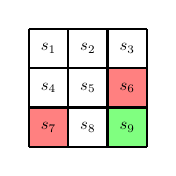
\begin{tikzpicture}[scale=0.5]
            % 填充指定格子为红色
            \fill[red!50] (2,1) rectangle (3,2); % 第2行第3列 (索引 (2,1))
            \fill[red!50] (0,0) rectangle (1,1); % 第3行第1列 (索引 (0,0))
            \fill[green!50] (2,0) rectangle (3,1); % 第3行第1列 (索引 (0,0))

            % 画3x3网格
            \draw[thick] (0,0) grid (3,3);
            
            % 标记状态编号 (行列索引)
            \foreach \x in {0,1,2} {
                \foreach \y in {0,1,2} {
                    \node at (\x+0.5, 2.5-\y){};
                }
            }

            % 在红色格子内写 "forbidden"
            \node[scale=0.6] at (0.5, 2.5) {$s_1$};
            \node[scale=0.6] at (1.5, 2.5) {$s_2$};
            \node[scale=0.6] at (2.5, 2.5) {$s_3$};
            \node[scale=0.6] at (0.5, 1.5) {$s_4$};
            \node[scale=0.6] at (1.5, 1.5) {$s_5$};
            \node[scale=0.6] at (2.5, 1.5) {$s_6$};
            \node[scale=0.6] at (0.5, 0.5) {$s_7$};
            \node[scale=0.6] at (1.5, 0.5) {$s_8$};
            \node[scale=0.6] at (2.5, 0.5) {$s_9$};

        \end{tikzpicture}
    \end{center}
    我们可以用一个表格去形容状态转移。(只能表述确定性的情况)
    % Please add the following required packages to your document preamble:
    \begin{table}[]
        \begin{tabular}{@{}llllll@{}}
        \toprule
            & $a_1$ & $a_2$ & $a_3$ & $a_4$ & $a_5$ \\ \midrule
        $s_1$ & $s_1$ & $s_2$ & $s_4$ & $s_1$ & $s_1$ \\
        $s_2$ & $s_2$ & $s_3$ & $s_5$ & $s_1$ & $s_2$ \\
        $s_3$ & $s_3$ & $s_3$ & $s_6$ & $s_2$ & $s_3$ \\
        $s_4$ & $s_1$ & $s_5$ & $s_7$ & $s_4$ & $s_4$ \\
        $s_5$ & $s_6$ & $s_8$ & $s_4$ & $s_2$ & $s_5$ \\
        $s_6$ & $s_3$ & $s_6$ & $s_9$ & $s_5$ & $s_6$ \\
        $s_7$ & $s_4$ & $s_8$ & $s_7$ & $s_7$ & $s_7$ \\
        $s_8$ & $s_5$ & $s_9$ & $s_8$ & $s_7$ & $s_8$ \\
        $s_9$ & $s_6$ & $s_9$ & $s_9$ & $s_8$ & $s_9$ \\ \bottomrule
        \end{tabular}
    \end{table}
\end{frame}

\begin{frame}{状态转移}
    \begin{center}
        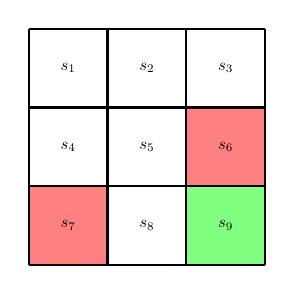
\begin{tikzpicture}
            % 填充指定格子为红色
            \fill[red!50] (2,1) rectangle (3,2); % 第2行第3列 (索引 (2,1))
            \fill[red!50] (0,0) rectangle (1,1); % 第3行第1列 (索引 (0,0))
            \fill[green!50] (2,0) rectangle (3,1); % 第3行第1列 (索引 (0,0))

            % 画3x3网格
            \draw[thick] (0,0) grid (3,3);
            
            % 标记状态编号 (行列索引)
            \foreach \x in {0,1,2} {
                \foreach \y in {0,1,2} {
                    \node at (\x+0.5, 2.5-\y){};
                }
            }

            % 在红色格子内写 "forbidden"
            \node[scale=0.6] at (0.5, 2.5) {$s_1$};
            \node[scale=0.6] at (1.5, 2.5) {$s_2$};
            \node[scale=0.6] at (2.5, 2.5) {$s_3$};
            \node[scale=0.6] at (0.5, 1.5) {$s_4$};
            \node[scale=0.6] at (1.5, 1.5) {$s_5$};
            \node[scale=0.6] at (2.5, 1.5) {$s_6$};
            \node[scale=0.6] at (0.5, 0.5) {$s_7$};
            \node[scale=0.6] at (1.5, 0.5) {$s_8$};
            \node[scale=0.6] at (2.5, 0.5) {$s_9$};

        \end{tikzpicture}
    \end{center}
    状态转移概率:使用概率来描述状态转移。
    \begin{itemize}
        \item 如果我们在状态$s_1$选择动作$a_2$,那么我们的下一个状态是$s_2$。
        \item 数学:
        \[
            \begin{split}
                P(s_2|s_1, a_2)&=1 \\
                P(s_i|s_1, a_2)&=0, \quad \forall i\neq 2
            \end{split}
        \]
    \end{itemize}
    这里是\alert{确定性}的情况,还有\alert{不确定性}的情况(比如说会刮风)。
\end{frame}

\begin{frame}{策略}
    \textbf{策略}告诉智能体在一个状态下应该选择什么样的动作。

    用箭头表示策略。
    \begin{center}
        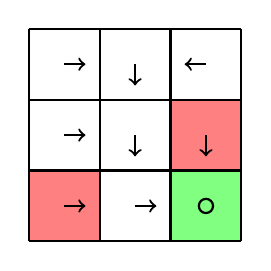
\begin{tikzpicture}[scale=0.9]
            % 填充指定格子为红色
            \fill[red!50] (2,1) rectangle (3,2); % 第2行第3列 (索引 (2,1))
            \fill[red!50] (0,0) rectangle (1,1); % 第3行第1列 (索引 (0,0))
            \fill[green!50] (2,0) rectangle (3,1); % 第3行第1列 (索引 (0,0))

            % 画3x3网格
            \draw[thick] (0,0) grid (3,3);
            
            % 标记状态编号 (行列索引)
            \foreach \x in {0,1,2} {
                \foreach \y in {0,1,2} {
                    \node at (\x+0.5, 2.5-\y){};
                }
            }
            
            % 绘制箭头表示策略
            % 示例:在格子中绘制箭头

            % 从 s_1 (0, 0) 向右的箭头
            \draw[->, thick] (0.5, 2.5) -- (0.8, 2.5); % 向右

            % 从 s_2 (1, 0) 向上
            \draw[->, thick] (1.5, 2.5) -- (1.5, 2.2); % 向上

            % 从 s_3 (2, 0) 向左
            \draw[->, thick] (2.5, 2.5) -- (2.2, 2.5); % 向左

            % 从 s_4 (0, 1) 向下
            \draw[->, thick] (0.5, 1.5) -- (0.8, 1.5); % 向下

            % 从 s_5 (1, 1) 向右
            \draw[->, thick] (1.5, 1.5) -- (1.5, 1.2); % 向右

            % 从 s_6 (2, 1) 向上
            \draw[->, thick] (2.5, 1.5) -- (2.5, 1.2); % 向上

            % 从 s_7 (0, 2) 向右
            \draw[->, thick] (0.5, 0.5) -- (0.8, 0.5); % 向右

            % 从 s_8 (1, 2) 向下
            \draw[->, thick] (1.5, 0.5) -- (1.8, 0.5); % 向下

            % 从 s_9 (2, 2) 向左
            \draw[thick] (2.5, 0.5) circle (0.1);
        \end{tikzpicture}
    \end{center}
    根据这个策略,我们可以从不同的出发点开始得到不同的轨迹。
    \begin{center}
        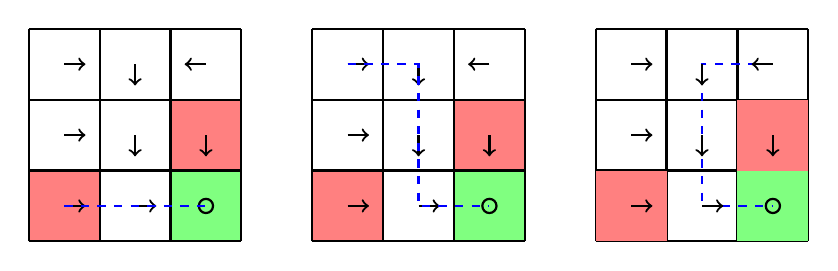
\begin{tikzpicture}[scale=0.9]
            % 填充指定格子为红色
            \fill[red!50] (2,1) rectangle (3,2); % 第2行第3列 (索引 (2,1))
            \fill[red!50] (0,0) rectangle (1,1); % 第3行第1列 (索引 (0,0))
            \fill[green!50] (2,0) rectangle (3,1); % 第3行第1列 (索引 (0,0))

            % 画3x3网格
            \draw[thick] (0,0) grid (3,3);
            
            % 标记状态编号 (行列索引)
            \foreach \x in {0,1,2} {
                \foreach \y in {0,1,2} {
                    \node at (\x+0.5, 2.5-\y){};
                }
            }
            
            % 从 s_1 (0, 0) 向右的箭头
            \draw[->, thick] (0.5, 2.5) -- (0.8, 2.5); % 向右

            % 从 s_2 (1, 0) 向上
            \draw[->, thick] (1.5, 2.5) -- (1.5, 2.2); % 向上

            % 从 s_3 (2, 0) 向左
            \draw[->, thick] (2.5, 2.5) -- (2.2, 2.5); % 向左

            % 从 s_4 (0, 1) 向下
            \draw[->, thick] (0.5, 1.5) -- (0.8, 1.5); % 向下

            % 从 s_5 (1, 1) 向右
            \draw[->, thick] (1.5, 1.5) -- (1.5, 1.2); % 向右

            % 从 s_6 (2, 1) 向上
            \draw[->, thick] (2.5, 1.5) -- (2.5, 1.2); % 向上

            % 从 s_7 (0, 2) 向右
            \draw[->, thick] (0.5, 0.5) -- (0.8, 0.5); % 向右

            % 从 s_8 (1, 2) 向下
            \draw[->, thick] (1.5, 0.5) -- (1.8, 0.5); % 向下

            % 从 s_9 (2, 2) 向左
            \draw[thick] (2.5, 0.5) circle (0.1);

            \draw[dashed, blue, thick] (0.5, 2.5) -- (1.5, 2.5) -- (1.5, 0.5) -- (2.5, 0.5);

            % 填充指定格子为红色
            \fill[red!50] (-2,1) rectangle (-1,2); % 第2行第3列 (索引 (2,1))
            \fill[red!50] (-4,0) rectangle (-3,1); % 第3行第1列 (索引 (0,0))
            \fill[green!50] (-2,0) rectangle (-1,1); % 第3行第1列 (索引 (0,0))

            % 画3x3网格
            \draw[thick] (-4,0) grid (-1,3);
            
            % 标记状态编号 (行列索引)
            \foreach \x in {0,1,2} {
                \foreach \y in {0,1,2} {
                    \node at (\x+0.5, 2.5-\y){};
                }
            }
            % 从 s_1 (0, 0) 向右的箭头
            \draw[->, thick] (-3.5, 2.5) -- (-3.2, 2.5); % 向右

            % 从 s_2 (1, 0) 向上
            \draw[->, thick] (-2.5, 2.5) -- (-2.5, 2.2); % 向上

            % 从 s_3 (2, 0) 向左
            \draw[->, thick] (-1.5, 2.5) -- (-1.8, 2.5); % 向左

            % 从 s_4 (0, 1) 向下
            \draw[->, thick] (-3.5, 1.5) -- (-3.2, 1.5); % 向下

            % 从 s_5 (1, 1) 向右
            \draw[->, thick] (-2.5, 1.5) -- (-2.5, 1.2); % 向右

            % 从 s_6 (2, 1) 向上
            \draw[->, thick] (-1.5, 1.5) -- (-1.5, 1.2); % 向上

            % 从 s_7 (0, 2) 向右
            \draw[->, thick] (-3.5, 0.5) -- (-3.2, 0.5); % 向右

            % 从 s_8 (1, 2) 向下
            \draw[->, thick] (-2.5, 0.5) -- (-2.2, 0.5); % 向下

            % 从 s_9 (2, 2) 向左
            \draw[thick] (-1.5, 0.5) circle (0.1);

            \draw[thick] (4,0) grid (7,3);
        
            % 填充指定格子为红色
            \fill[red!50] (6,1) rectangle (7,2); % 第2行第3列 (索引 (2,1))
            \fill[red!50] (4,0) rectangle (5,1); % 第3行第1列 (索引 (0,0))
            \fill[green!50] (6,0) rectangle (7,1); % 第3行第1列 (索引 (0,0))

            % 画3x3网格
            
            \draw[dashed, blue, thick] (6.5, 2.5) -- (5.5, 2.5) -- (5.5, 0.5) -- (6.5, 0.5);
            
            % 标记状态编号 (行列索引)
            \foreach \x in {0,1,2} {
                \foreach \y in {0,1,2} {
                    \node at (\x+0.5, 2.5-\y){};
                }
            }
            % 从 s_1 (0, 0) 向右的箭头
            \draw[->, thick] (4.5, 2.5) -- (4.8, 2.5); % 向右

            % 从 s_2 (1, 0) 向上
            \draw[->, thick] (5.5, 2.5) -- (5.5, 2.2); % 向上

            % 从 s_3 (2, 0) 向左
            \draw[->, thick] (6.5, 2.5) -- (6.2, 2.5); % 向左

            % 从 s_4 (0, 1) 向下
            \draw[->, thick] (4.5, 1.5) -- (4.8, 1.5); % 向下

            % 从 s_5 (1, 1) 向右
            \draw[->, thick] (5.5, 1.5) -- (5.5, 1.2); % 向右

            % 从 s_6 (2, 1) 向上
            \draw[->, thick] (6.5, 1.5) -- (6.5, 1.2); % 向上

            % 从 s_7 (0, 2) 向右
            \draw[->, thick] (4.5, 0.5) -- (4.8, 0.5); % 向右

            % 从 s_8 (1, 2) 向下
            \draw[->, thick] (5.5, 0.5) -- (5.8, 0.5); % 向下

            % 从 s_9 (2, 2) 向左
            \draw[thick] (6.5, 0.5) circle (0.1);

            \draw[dashed, blue, thick] (-3.5, 0.5) -- (-1.5, 0.5);
            
        \end{tikzpicture}
    \end{center}

\end{frame}

\begin{frame}{策略}
    \begin{center}
        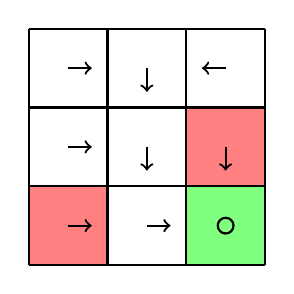
\begin{tikzpicture}
            % 填充指定格子为红色
            \fill[red!50] (2,1) rectangle (3,2); % 第2行第3列 (索引 (2,1))
            \fill[red!50] (0,0) rectangle (1,1); % 第3行第1列 (索引 (0,0))
            \fill[green!50] (2,0) rectangle (3,1); % 第3行第1列 (索引 (0,0))

            % 画3x3网格
            \draw[thick] (0,0) grid (3,3);
            
            % 标记状态编号 (行列索引)
            \foreach \x in {0,1,2} {
                \foreach \y in {0,1,2} {
                    \node at (\x+0.5, 2.5-\y){};
                }
            }
            
            % 绘制箭头表示策略
            % 示例:在格子中绘制箭头

            % 从 s_1 (0, 0) 向右的箭头
            \draw[->, thick] (0.5, 2.5) -- (0.8, 2.5); % 向右

            % 从 s_2 (1, 0) 向上
            \draw[->, thick] (1.5, 2.5) -- (1.5, 2.2); % 向上

            % 从 s_3 (2, 0) 向左
            \draw[->, thick] (2.5, 2.5) -- (2.2, 2.5); % 向左

            % 从 s_4 (0, 1) 向下
            \draw[->, thick] (0.5, 1.5) -- (0.8, 1.5); % 向下

            % 从 s_5 (1, 1) 向右
            \draw[->, thick] (1.5, 1.5) -- (1.5, 1.2); % 向右

            % 从 s_6 (2, 1) 向上
            \draw[->, thick] (2.5, 1.5) -- (2.5, 1.2); % 向上

            % 从 s_7 (0, 2) 向右
            \draw[->, thick] (0.5, 0.5) -- (0.8, 0.5); % 向右

            % 从 s_8 (1, 2) 向下
            \draw[->, thick] (1.5, 0.5) -- (1.8, 0.5); % 向下

            % 从 s_9 (2, 2) 向左
            \draw[thick] (2.5, 0.5) circle (0.1);
        \end{tikzpicture}
    \end{center}
    数学表示:用条件概率表示策略。

    对于$s_1$而言:
    \[
        \begin{aligned}
            \pi(a_1|s_1) = 0 \\
            \pi(a_2|s_1) = 1 \\
            \pi(a_3|s_1) = 0 \\
            \pi(a_4|s_1) = 0 \\
            \pi(a_5|s_1) = 0 \\
        \end{aligned}
    \]
    这是一个\alert{确定性}策略。
\end{frame}

\begin{frame}{策略}
    随机策略:
    \begin{center}
        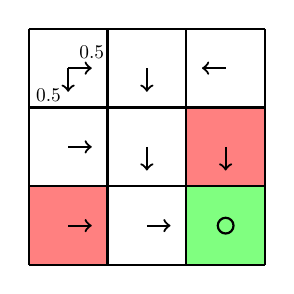
\begin{tikzpicture}
            % 填充指定格子为红色
            \fill[red!50] (2,1) rectangle (3,2); % 第2行第3列 (索引 (2,1))
            \fill[red!50] (0,0) rectangle (1,1); % 第3行第1列 (索引 (0,0))
            \fill[green!50] (2,0) rectangle (3,1); % 第3行第1列 (索引 (0,0))

            % 画3x3网格
            \draw[thick] (0,0) grid (3,3);
            
            % 标记状态编号 (行列索引)
            \foreach \x in {0,1,2} {
                \foreach \y in {0,1,2} {
                    \node at (\x+0.5, 2.5-\y){};
                }
            }
            
            % 绘制箭头表示策略
            % 示例:在格子中绘制箭头

            % 从 s_1 (0, 0) 向右的箭头
            \draw[->, thick] (0.5, 2.5) -- (0.8, 2.5); % 向右
            \node[scale=0.7] at (0.8, 2.7) {0.5}; % 在箭头上方标注 50%
            \draw[->, thick] (0.5, 2.5) -- (0.5, 2.2);
            \node[scale=0.7] at (0.25, 2.15) {0.5}; % 在箭头右侧标注 50%

           % 从 s_2 (1, 0) 向上
           \draw[->, thick] (1.5, 2.5) -- (1.5, 2.2); % 向上

           % 从 s_3 (2, 0) 向左
           \draw[->, thick] (2.5, 2.5) -- (2.2, 2.5); % 向左

           % 从 s_4 (0, 1) 向下
           \draw[->, thick] (0.5, 1.5) -- (0.8, 1.5); % 向下

           % 从 s_5 (1, 1) 向右
           \draw[->, thick] (1.5, 1.5) -- (1.5, 1.2); % 向右

           % 从 s_6 (2, 1) 向上
           \draw[->, thick] (2.5, 1.5) -- (2.5, 1.2); % 向上

           % 从 s_7 (0, 2) 向右
           \draw[->, thick] (0.5, 0.5) -- (0.8, 0.5); % 向右

           % 从 s_8 (1, 2) 向下
           \draw[->, thick] (1.5, 0.5) -- (1.8, 0.5); % 向下

           % 从 s_9 (2, 2) 向左
           \draw[thick] (2.5, 0.5) circle (0.1);
        \end{tikzpicture}
    \end{center}

    在这个策略中,对于$s_1$而言:
    \[
        \begin{aligned}
            \pi(a_1|s_1) &= 0 \\
            \pi(a_2|s_1) &= 0.5 \\
            \pi(a_3|s_1) &= 0.5 \\
            \pi(a_4|s_1) &= 0 \\
            \pi(a_5|s_1) &= 0 \\
        \end{aligned}
    \]
\end{frame}

\begin{frame}{策略}
    \begin{center}
        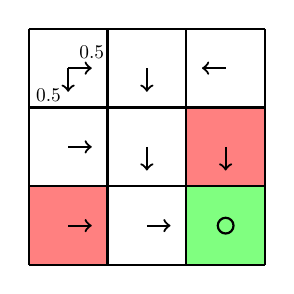
\begin{tikzpicture}
            % 填充指定格子为红色
            \fill[red!50] (2,1) rectangle (3,2); % 第2行第3列 (索引 (2,1))
            \fill[red!50] (0,0) rectangle (1,1); % 第3行第1列 (索引 (0,0))
            \fill[green!50] (2,0) rectangle (3,1); % 第3行第1列 (索引 (0,0))

            % 画3x3网格
            \draw[thick] (0,0) grid (3,3);
            
            % 标记状态编号 (行列索引)
            \foreach \x in {0,1,2} {
                \foreach \y in {0,1,2} {
                    \node at (\x+0.5, 2.5-\y){};
                }
            }
            
            % 绘制箭头表示策略
            % 示例:在格子中绘制箭头

            % 从 s_1 (0, 0) 向右的箭头
            \draw[->, thick] (0.5, 2.5) -- (0.8, 2.5); % 向右
            \node[scale=0.7] at (0.8, 2.7) {0.5}; % 在箭头上方标注 50%
            \draw[->, thick] (0.5, 2.5) -- (0.5, 2.2);
            \node[scale=0.7] at (0.25, 2.15) {0.5}; % 在箭头右侧标注 50%

           % 从 s_2 (1, 0) 向上
           \draw[->, thick] (1.5, 2.5) -- (1.5, 2.2); % 向上

           % 从 s_3 (2, 0) 向左
           \draw[->, thick] (2.5, 2.5) -- (2.2, 2.5); % 向左

           % 从 s_4 (0, 1) 向下
           \draw[->, thick] (0.5, 1.5) -- (0.8, 1.5); % 向下

           % 从 s_5 (1, 1) 向右
           \draw[->, thick] (1.5, 1.5) -- (1.5, 1.2); % 向右

           % 从 s_6 (2, 1) 向上
           \draw[->, thick] (2.5, 1.5) -- (2.5, 1.2); % 向上

           % 从 s_7 (0, 2) 向右
           \draw[->, thick] (0.5, 0.5) -- (0.8, 0.5); % 向右

           % 从 s_8 (1, 2) 向下
           \draw[->, thick] (1.5, 0.5) -- (1.8, 0.5); % 向下

           % 从 s_9 (2, 2) 向左
           \draw[thick] (2.5, 0.5) circle (0.1);
        \end{tikzpicture}
    \end{center}
    用表格形式表示一个策略。
    \begin{table}[]
        \begin{tabular}{@{}llllll@{}}
        \toprule
            & $a_1$ & $a_2$ & $a_3$ & $a_4$ & $a_5$ \\ \midrule
        $s_1$ & $0$ & $0.5$ & $0.5$ & $0$ & $0$ \\
        $s_2$ & $0$ & $0$ & $1$ & $0$ & $0$ \\
        $\cdots$ &  &  & $\cdots$ & & \\
        $s_9$ & $0$ & $0$ & $0$ & $0$ & $1$ \\ \bottomrule
        \end{tabular}
    \end{table}
    这样既可以表示确定性策略,也可以表示随机策略。
\end{frame}

\begin{frame}{奖励}
    \textbf{奖励}是一个智能体做出动作之后得到的一个实数。
    \begin{itemize}
        \item 一个\alert{正数}的奖励值鼓励智能体做这样的动作;
        \item 一个\alert{负数}的奖励值惩罚智能体做这样的动作。
    \end{itemize}
    问题:
    \begin{itemize}
        \item 可以让正数代表惩罚,负数代表鼓励吗?
        \begin{itemize}
            \item 可以。
            \item 在这种情况下,奖励被称作\alert{代价}。
        \end{itemize}
        \item 奖励值为0会怎么样?
        \begin{itemize}
            \item 只有相对奖励值才有意义,绝对的奖励值没有意义。
            \item $r=\{+1,-1\}$变成$r=\{+2,0\}$并不会对策略有任何影响。
        \end{itemize}
    \end{itemize}
\end{frame}

\begin{frame}{奖励}
    \begin{center}
        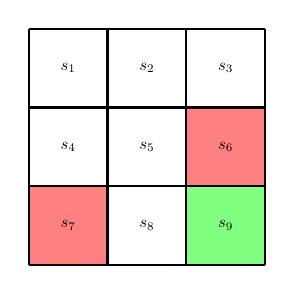
\begin{tikzpicture}
            % 填充指定格子为红色
            \fill[red!50] (2,1) rectangle (3,2); % 第2行第3列 (索引 (2,1))
            \fill[red!50] (0,0) rectangle (1,1); % 第3行第1列 (索引 (0,0))
            \fill[green!50] (2,0) rectangle (3,1); % 第3行第1列 (索引 (0,0))

            % 画3x3网格
            \draw[thick] (0,0) grid (3,3);
            
            % 标记状态编号 (行列索引)
            \foreach \x in {0,1,2} {
                \foreach \y in {0,1,2} {
                    \node at (\x+0.5, 2.5-\y){};
                }
            }

            % 在红色格子内写 "forbidden"
            \node[scale=0.6] at (0.5, 2.5) {$s_1$};
            \node[scale=0.6] at (1.5, 2.5) {$s_2$};
            \node[scale=0.6] at (2.5, 2.5) {$s_3$};
            \node[scale=0.6] at (0.5, 1.5) {$s_4$};
            \node[scale=0.6] at (1.5, 1.5) {$s_5$};
            \node[scale=0.6] at (2.5, 1.5) {$s_6$};
            \node[scale=0.6] at (0.5, 0.5) {$s_7$};
            \node[scale=0.6] at (1.5, 0.5) {$s_8$};
            \node[scale=0.6] at (2.5, 0.5) {$s_9$};

        \end{tikzpicture}
    \end{center}
    在网格世界中,我们可以这样设置奖励:
    \begin{itemize}
        \item 如果智能体撞墙了,那么奖励值$r_{\text{bound}}=-1$;
        \item 如果智能体试图进入一个禁止通过的区域,那么奖励值$r_{\text{forbidden}}=-1$
        \item 如果智能体到达终点,那么奖励值$r_{\text{target}}=+1$
        \item 其他情况奖励值$r=0$
    \end{itemize}
    奖励值的存在可以让我们人类引导智能体按照我们想要的方式行动。

    比如上述奖励的设置可以让智能体尽量不要撞墙或者试图进入禁止通过的区域。
\end{frame}

\begin{frame}{奖励}
    \begin{center}
        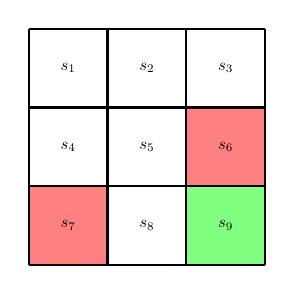
\begin{tikzpicture}
            % 填充指定格子为红色
            \fill[red!50] (2,1) rectangle (3,2); % 第2行第3列 (索引 (2,1))
            \fill[red!50] (0,0) rectangle (1,1); % 第3行第1列 (索引 (0,0))
            \fill[green!50] (2,0) rectangle (3,1); % 第3行第1列 (索引 (0,0))

            % 画3x3网格
            \draw[thick] (0,0) grid (3,3);
            
            % 标记状态编号 (行列索引)
            \foreach \x in {0,1,2} {
                \foreach \y in {0,1,2} {
                    \node at (\x+0.5, 2.5-\y){};
                }
            }

            % 在红色格子内写 "forbidden"
            \node[scale=0.6] at (0.5, 2.5) {$s_1$};
            \node[scale=0.6] at (1.5, 2.5) {$s_2$};
            \node[scale=0.6] at (2.5, 2.5) {$s_3$};
            \node[scale=0.6] at (0.5, 1.5) {$s_4$};
            \node[scale=0.6] at (1.5, 1.5) {$s_5$};
            \node[scale=0.6] at (2.5, 1.5) {$s_6$};
            \node[scale=0.6] at (0.5, 0.5) {$s_7$};
            \node[scale=0.6] at (1.5, 0.5) {$s_8$};
            \node[scale=0.6] at (2.5, 0.5) {$s_9$};

        \end{tikzpicture}
    \end{center}
    用表格形式表示奖励机制。
    \begin{table}[]
        \begin{tabular}{@{}llllll@{}}
        \toprule
            & $a_1$ & $a_2$ & $a_3$ & $a_4$ & $a_5$ \\ \midrule
        $s_1$ & $r_{\text{bound}}$ & $0$ & $0$ & $r_{\text{bound}}$ & $0$ \\
        $s_2$ & $r_{\text{bound}}$ & $0$ & $0$ & $0$ & $0$ \\
        $\cdots$ &  &  & $\cdots$ & & \\
        $s_9$ & $r_{\text{forbidden}}$ & $r_{\text{bound}}$ & $r_{\text{bound}}$ & $0$ & $r_{\text{target}}$ \\ \bottomrule
        \end{tabular}
    \end{table}
    只能用来表示确定性的奖励机制。
\end{frame}

\begin{frame}{奖励}
    \begin{center}
        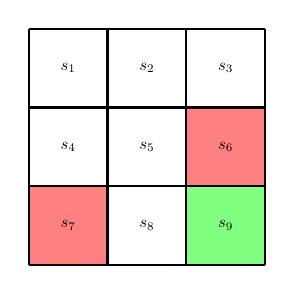
\begin{tikzpicture}
            % 填充指定格子为红色
            \fill[red!50] (2,1) rectangle (3,2); % 第2行第3列 (索引 (2,1))
            \fill[red!50] (0,0) rectangle (1,1); % 第3行第1列 (索引 (0,0))
            \fill[green!50] (2,0) rectangle (3,1); % 第3行第1列 (索引 (0,0))

            % 画3x3网格
            \draw[thick] (0,0) grid (3,3);
            
            % 标记状态编号 (行列索引)
            \foreach \x in {0,1,2} {
                \foreach \y in {0,1,2} {
                    \node at (\x+0.5, 2.5-\y){};
                }
            }

            % 在红色格子内写 "forbidden"
            \node[scale=0.6] at (0.5, 2.5) {$s_1$};
            \node[scale=0.6] at (1.5, 2.5) {$s_2$};
            \node[scale=0.6] at (2.5, 2.5) {$s_3$};
            \node[scale=0.6] at (0.5, 1.5) {$s_4$};
            \node[scale=0.6] at (1.5, 1.5) {$s_5$};
            \node[scale=0.6] at (2.5, 1.5) {$s_6$};
            \node[scale=0.6] at (0.5, 0.5) {$s_7$};
            \node[scale=0.6] at (1.5, 0.5) {$s_8$};
            \node[scale=0.6] at (2.5, 0.5) {$s_9$};

        \end{tikzpicture}
    \end{center}
    数学形式:条件概率
    \begin{itemize}
        \item 在$s_1$我们选择动作$a_1$奖励会是-1。
        \item $p(r=-1|s_1, a_1)=1$且$p(r\neq-1|s_1,a_1)=0$
    \end{itemize}
    值得注意的是:

    在一个确定的状态执行一个确定的动作,得到的奖励并不是确定的。比如努力学习一定会得到奖励,但是具体多少是不一定的。
\end{frame}

\begin{frame}{轨迹和回报}
    \begin{center}
        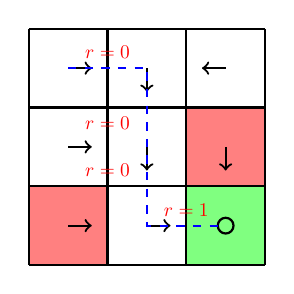
\begin{tikzpicture}
            % 填充指定格子为红色
            \fill[red!50] (2,1) rectangle (3,2); % 第2行第3列 (索引 (2,1))
            \fill[red!50] (0,0) rectangle (1,1); % 第3行第1列 (索引 (0,0))
            \fill[green!50] (2,0) rectangle (3,1); % 第3行第1列 (索引 (0,0))

            % 画3x3网格
            \draw[thick] (0,0) grid (3,3);
            
            % 标记状态编号 (行列索引)
            \foreach \x in {0,1,2} {
                \foreach \y in {0,1,2} {
                    \node at (\x+0.5, 2.5-\y){};
                }
            }
            
            % 绘制箭头表示策略
            % 示例:在格子中绘制箭头

            % 从 s_1 (0, 0) 向右的箭头
            \draw[->, thick] (0.5, 2.5) -- (0.8, 2.5); % 向右

            % 从 s_2 (1, 0) 向上
            \draw[->, thick] (1.5, 2.5) -- (1.5, 2.2); % 向上

            % 从 s_3 (2, 0) 向左
            \draw[->, thick] (2.5, 2.5) -- (2.2, 2.5); % 向左

            % 从 s_4 (0, 1) 向下
            \draw[->, thick] (0.5, 1.5) -- (0.8, 1.5); % 向下

            % 从 s_5 (1, 1) 向右
            \draw[->, thick] (1.5, 1.5) -- (1.5, 1.2); % 向右

            % 从 s_6 (2, 1) 向上
            \draw[->, thick] (2.5, 1.5) -- (2.5, 1.2); % 向上

            % 从 s_7 (0, 2) 向右
            \draw[->, thick] (0.5, 0.5) -- (0.8, 0.5); % 向右

            % 从 s_8 (1, 2) 向下
            \draw[->, thick] (1.5, 0.5) -- (1.8, 0.5); % 向下

            % 从 s_9 (2, 2) 向左
            \draw[thick] (2.5, 0.5) circle (0.1);
            \draw[dashed, blue, thick] (0.5, 2.5) -- (1.5, 2.5) -- (1.5, 0.5) -- (2.5, 0.5);
            \node[scale=0.7, color=red] at (1, 2.7) {$r=0$};
            \node[scale=0.7, color=red] at (1, 1.8) {$r=0$};
            \node[scale=0.7, color=red] at (1, 1.2) {$r=0$};
            \node[scale=0.7, color=red] at (2, 0.7) {$r=1$};
        \end{tikzpicture}
    \end{center}

    \textbf{轨迹}是一个状态-动作-奖励链。
    \[
        s_1\overset{a_2}{\underset{r=0}{\longrightarrow}} s_2\overset{a_3}{\underset{r=0}{\longrightarrow}} s_5\overset{a_3}{\underset{r=0}{\longrightarrow}} s_8\overset{a_2}{\underset{r=1}{\longrightarrow}} s_9
    \]
    \textbf{回报}是这一条轨迹上所有的奖励之和。
    \[
        \text{return}=0+0+0+1=1
    \]
\end{frame}

\begin{frame}{轨迹和回报}
    \begin{center}
        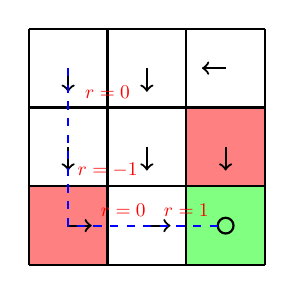
\begin{tikzpicture}
            % 填充指定格子为红色
            \fill[red!50] (2,1) rectangle (3,2); % 第2行第3列 (索引 (2,1))
            \fill[red!50] (0,0) rectangle (1,1); % 第3行第1列 (索引 (0,0))
            \fill[green!50] (2,0) rectangle (3,1); % 第3行第1列 (索引 (0,0))

            % 画3x3网格
            \draw[thick] (0,0) grid (3,3);
            
            % 标记状态编号 (行列索引)
            \foreach \x in {0,1,2} {
                \foreach \y in {0,1,2} {
                    \node at (\x+0.5, 2.5-\y){};
                }
            }
            
            % 绘制箭头表示策略
            % 示例:在格子中绘制箭头

            % 从 s_1 (0, 0) 向右的箭头
            \draw[->, thick] (0.5, 2.5) -- (0.5, 2.2); % 向右

            % 从 s_2 (1, 0) 向上
            \draw[->, thick] (1.5, 2.5) -- (1.5, 2.2); % 向上

            % 从 s_3 (2, 0) 向左
            \draw[->, thick] (2.5, 2.5) -- (2.2, 2.5); % 向左

            % 从 s_4 (0, 1) 向下
            \draw[->, thick] (0.5, 1.5) -- (0.5, 1.2); % 向下

            % 从 s_5 (1, 1) 向右
            \draw[->, thick] (1.5, 1.5) -- (1.5, 1.2); % 向右

            % 从 s_6 (2, 1) 向上
            \draw[->, thick] (2.5, 1.5) -- (2.5, 1.2); % 向上

            % 从 s_7 (0, 2) 向右
            \draw[->, thick] (0.5, 0.5) -- (0.8, 0.5); % 向右

            % 从 s_8 (1, 2) 向下
            \draw[->, thick] (1.5, 0.5) -- (1.8, 0.5); % 向下

            % 从 s_9 (2, 2) 向左
            \draw[thick] (2.5, 0.5) circle (0.1);
            \draw[dashed, blue, thick] (0.5, 2.5) -- (0.5, 0.5) -- (2.5, 0.5);
            \node[scale=0.7, color=red] at (1, 2.2) {$r=0$};
            \node[scale=0.7, color=red] at (1, 1.2) {$r=-1$};
            \node[scale=0.7, color=red] at (1.2, 0.7) {$r=0$};
            \node[scale=0.7, color=red] at (2, 0.7) {$r=1$};
        \end{tikzpicture}
    \end{center}

    不同的策略会有不同的轨迹
    \[
        s_1\overset{a_3}{\underset{r=0}{\longrightarrow}} s_4\overset{a_3}{\underset{r=-1}{\longrightarrow}} s_7\overset{a_2}{\underset{r=0}{\longrightarrow}} s_8\overset{a_2}{\underset{r=1}{\longrightarrow}} s_9
    \]
    \textbf{回报}是这一条轨迹上所有的奖励之和。
    \[
        \text{return}=0+(-1)+0+1=0
    \]
\end{frame}

\begin{frame}{轨迹和回报}
    \begin{center}
        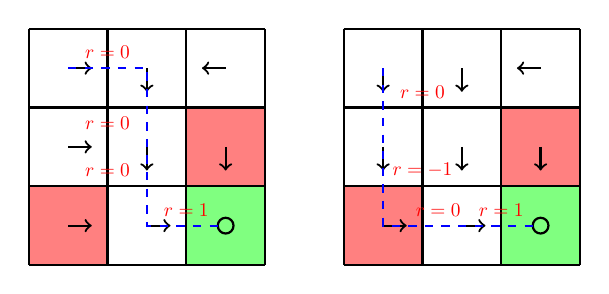
\begin{tikzpicture}
            % 填充指定格子为红色
            \fill[red!50] (2,1) rectangle (3,2); % 第2行第3列 (索引 (2,1))
            \fill[red!50] (0,0) rectangle (1,1); % 第3行第1列 (索引 (0,0))
            \fill[green!50] (2,0) rectangle (3,1); % 第3行第1列 (索引 (0,0))

            % 画3x3网格
            \draw[thick] (0,0) grid (3,3);
            
            % 标记状态编号 (行列索引)
            \foreach \x in {0,1,2} {
                \foreach \y in {0,1,2} {
                    \node at (\x+0.5, 2.5-\y){};
                }
            }
            
            % 绘制箭头表示策略
            % 示例:在格子中绘制箭头

            % 从 s_1 (0, 0) 向右的箭头
            \draw[->, thick] (0.5, 2.5) -- (0.8, 2.5); % 向右

            % 从 s_2 (1, 0) 向上
            \draw[->, thick] (1.5, 2.5) -- (1.5, 2.2); % 向上

            % 从 s_3 (2, 0) 向左
            \draw[->, thick] (2.5, 2.5) -- (2.2, 2.5); % 向左

            % 从 s_4 (0, 1) 向下
            \draw[->, thick] (0.5, 1.5) -- (0.8, 1.5); % 向下

            % 从 s_5 (1, 1) 向右
            \draw[->, thick] (1.5, 1.5) -- (1.5, 1.2); % 向右

            % 从 s_6 (2, 1) 向上
            \draw[->, thick] (2.5, 1.5) -- (2.5, 1.2); % 向上

            % 从 s_7 (0, 2) 向右
            \draw[->, thick] (0.5, 0.5) -- (0.8, 0.5); % 向右

            % 从 s_8 (1, 2) 向下
            \draw[->, thick] (1.5, 0.5) -- (1.8, 0.5); % 向下

            % 从 s_9 (2, 2) 向左
            \draw[thick] (2.5, 0.5) circle (0.1);
            \draw[dashed, blue, thick] (0.5, 2.5) -- (1.5, 2.5) -- (1.5, 0.5) -- (2.5, 0.5);
            \node[scale=0.7, color=red] at (1, 2.7) {$r=0$};
            \node[scale=0.7, color=red] at (1, 1.8) {$r=0$};
            \node[scale=0.7, color=red] at (1, 1.2) {$r=0$};
            \node[scale=0.7, color=red] at (2, 0.7) {$r=1$};

            % 填充指定格子为红色
            \fill[red!50] (6,1) rectangle (7,2); % 第2行第3列 (索引 (2,1))
            \fill[red!50] (4,0) rectangle (5,1); % 第3行第1列 (索引 (0,0))
            \fill[green!50] (6,0) rectangle (7,1); % 第3行第1列 (索引 (0,0))

            % 画3x3网格
            \draw[thick] (4,0) grid (7,3);
            
            % 标记状态编号 (行列索引)
            \foreach \x in {0,1,2} {
                \foreach \y in {0,1,2} {
                    \node at (\x+0.5, 2.5-\y){};
                }
            }
            
            % 绘制箭头表示策略
            % 示例:在格子中绘制箭头

            % 从 s_1 (0, 0) 向右的箭头
            \draw[->, thick] (4.5, 2.5) -- (4.5, 2.2); % 向右

            % 从 s_2 (1, 0) 向上
            \draw[->, thick] (5.5, 2.5) -- (5.5, 2.2); % 向上

            % 从 s_3 (2, 0) 向左
            \draw[->, thick] (6.5, 2.5) -- (6.2, 2.5); % 向左

            % 从 s_4 (0, 1) 向下
            \draw[->, thick] (4.5, 1.5) -- (4.5, 1.2); % 向下

            % 从 s_5 (1, 1) 向右
            \draw[->, thick] (5.5, 1.5) -- (5.5, 1.2); % 向右

            % 从 s_6 (2, 1) 向上
            \draw[->, thick] (6.5, 1.5) -- (6.5, 1.2); % 向上

            % 从 s_7 (0, 2) 向右
            \draw[->, thick] (4.5, 0.5) -- (4.8, 0.5); % 向右

            % 从 s_8 (1, 2) 向下
            \draw[->, thick] (5.5, 0.5) -- (5.8, 0.5); % 向下

            % 从 s_9 (2, 2) 向左
            \draw[thick] (6.5, 0.5) circle (0.1);
            \draw[dashed, blue, thick] (4.5, 2.5) -- (4.5, 0.5) -- (6.5, 0.5);
            \node[scale=0.7, color=red] at (5, 2.2) {$r=0$};
            \node[scale=0.7, color=red] at (5, 1.2) {$r=-1$};
            \node[scale=0.7, color=red] at (5.2, 0.7) {$r=0$};
            \node[scale=0.7, color=red] at (6, 0.7) {$r=1$};
        \end{tikzpicture}
    \end{center}

    哪个策略更好一点?
    \begin{itemize}
        \item 第一个更好,因为它没有经过禁止通过的区域;
        \item 第一个更好,因为它的\alert{回报}更高。
    \end{itemize}
    回报可以衡量一个策略的好坏。
\end{frame}

\begin{frame}{折扣回报}
    \begin{center}
        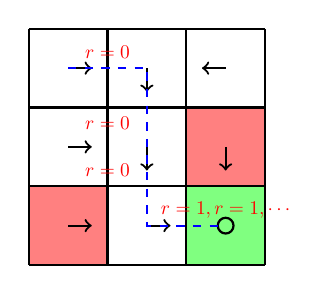
\begin{tikzpicture}
            % 填充指定格子为红色
            \fill[red!50] (2,1) rectangle (3,2); % 第2行第3列 (索引 (2,1))
            \fill[red!50] (0,0) rectangle (1,1); % 第3行第1列 (索引 (0,0))
            \fill[green!50] (2,0) rectangle (3,1); % 第3行第1列 (索引 (0,0))

            % 画3x3网格
            \draw[thick] (0,0) grid (3,3);
            
            % 标记状态编号 (行列索引)
            \foreach \x in {0,1,2} {
                \foreach \y in {0,1,2} {
                    \node at (\x+0.5, 2.5-\y){};
                }
            }
            
            % 绘制箭头表示策略
            % 示例:在格子中绘制箭头

            % 从 s_1 (0, 0) 向右的箭头
            \draw[->, thick] (0.5, 2.5) -- (0.8, 2.5); % 向右

            % 从 s_2 (1, 0) 向上
            \draw[->, thick] (1.5, 2.5) -- (1.5, 2.2); % 向上

            % 从 s_3 (2, 0) 向左
            \draw[->, thick] (2.5, 2.5) -- (2.2, 2.5); % 向左

            % 从 s_4 (0, 1) 向下
            \draw[->, thick] (0.5, 1.5) -- (0.8, 1.5); % 向下

            % 从 s_5 (1, 1) 向右
            \draw[->, thick] (1.5, 1.5) -- (1.5, 1.2); % 向右

            % 从 s_6 (2, 1) 向上
            \draw[->, thick] (2.5, 1.5) -- (2.5, 1.2); % 向上

            % 从 s_7 (0, 2) 向右
            \draw[->, thick] (0.5, 0.5) -- (0.8, 0.5); % 向右

            % 从 s_8 (1, 2) 向下
            \draw[->, thick] (1.5, 0.5) -- (1.8, 0.5); % 向下

            % 从 s_9 (2, 2) 向左
            \draw[thick] (2.5, 0.5) circle (0.1);
            \draw[dashed, blue, thick] (0.5, 2.5) -- (1.5, 2.5) -- (1.5, 0.5) -- (2.5, 0.5);
            \node[scale=0.7, color=red] at (1, 2.7) {$r=0$};
            \node[scale=0.7, color=red] at (1, 1.8) {$r=0$};
            \node[scale=0.7, color=red] at (1, 1.2) {$r=0$};
            \node[scale=0.7, color=red] at (2.5, 0.7) {$r=1,r=1,\cdots$};
        \end{tikzpicture}
    \end{center}
    轨迹可能是无限的:
    \[
        s_1\overset{a_2}{\underset{r=0}{\longrightarrow}} s_2\overset{a_3}{\underset{r=0}{\longrightarrow}} s_5\overset{a_3}{\underset{r=0}{\longrightarrow}} s_8\overset{a_2}{\underset{r=1}{\longrightarrow}} s_9\overset{a_5}{\underset{r=1}{\longrightarrow}} s_9\overset{a_5}{\underset{r=1}{\longrightarrow}} s_9\cdots
    \]
    回报是:
    \[
        \text{return}=0+0+0+1+1+\cdots
    \]
    这样的回报是发散的,是属于一种无效的定义。
\end{frame}

\begin{frame}{折扣回报}
    \begin{center}
        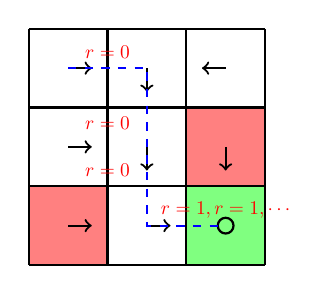
\begin{tikzpicture}
            % 填充指定格子为红色
            \fill[red!50] (2,1) rectangle (3,2); % 第2行第3列 (索引 (2,1))
            \fill[red!50] (0,0) rectangle (1,1); % 第3行第1列 (索引 (0,0))
            \fill[green!50] (2,0) rectangle (3,1); % 第3行第1列 (索引 (0,0))

            % 画3x3网格
            \draw[thick] (0,0) grid (3,3);
            
            % 标记状态编号 (行列索引)
            \foreach \x in {0,1,2} {
                \foreach \y in {0,1,2} {
                    \node at (\x+0.5, 2.5-\y){};
                }
            }
            
            % 绘制箭头表示策略
            % 示例:在格子中绘制箭头

            % 从 s_1 (0, 0) 向右的箭头
            \draw[->, thick] (0.5, 2.5) -- (0.8, 2.5); % 向右

            % 从 s_2 (1, 0) 向上
            \draw[->, thick] (1.5, 2.5) -- (1.5, 2.2); % 向上

            % 从 s_3 (2, 0) 向左
            \draw[->, thick] (2.5, 2.5) -- (2.2, 2.5); % 向左

            % 从 s_4 (0, 1) 向下
            \draw[->, thick] (0.5, 1.5) -- (0.8, 1.5); % 向下

            % 从 s_5 (1, 1) 向右
            \draw[->, thick] (1.5, 1.5) -- (1.5, 1.2); % 向右

            % 从 s_6 (2, 1) 向上
            \draw[->, thick] (2.5, 1.5) -- (2.5, 1.2); % 向上

            % 从 s_7 (0, 2) 向右
            \draw[->, thick] (0.5, 0.5) -- (0.8, 0.5); % 向右

            % 从 s_8 (1, 2) 向下
            \draw[->, thick] (1.5, 0.5) -- (1.8, 0.5); % 向下

            % 从 s_9 (2, 2) 向左
            \draw[thick] (2.5, 0.5) circle (0.1);
            \draw[dashed, blue, thick] (0.5, 2.5) -- (1.5, 2.5) -- (1.5, 0.5) -- (2.5, 0.5);
            \node[scale=0.7, color=red] at (1, 2.7) {$r=0$};
            \node[scale=0.7, color=red] at (1, 1.8) {$r=0$};
            \node[scale=0.7, color=red] at (1, 1.2) {$r=0$};
            \node[scale=0.7, color=red] at (2.5, 0.7) {$r=1,r=1,\cdots$};
        \end{tikzpicture}
    \end{center}
    需要引入一种折扣系数$\gamma\in(0,1)$:
    \[
        \begin{aligned}
            \text{折扣回报}&=0+\gamma 0 +\gamma^2 0+\gamma^3 1 +\gamma^41+\gamma^51+\cdots\\
            &=\gamma^3(1+\gamma+\gamma^2+\cdots)=\gamma^3\frac{1}{1-\gamma}
        \end{aligned}
    \]
    $\gamma$的作用:1)求和会变成一个有限的数;2)可以用来平衡短期收益和长期收益。
    \begin{itemize}
        \item 如果$\gamma$更接近0,那么折扣回报会更依赖于短期收益;
        \item 如果$\gamma$更接近1,那么折扣回报会更依赖于长期收益。
    \end{itemize}
\end{frame}

\begin{frame}{马尔可夫决策过程(MDP)}
    MDP的关键要素:
    \begin{itemize}
        \item 集合:
        \begin{itemize}
            \item 状态:状态集合$\mathcal{S}$
            \item 动作:动作集合$\mathcal{A}(s)$是与状态$s\in \mathcal{S}$关联的
            \item 奖励:奖励集合$\mathcal{R}(s,a)$
        \end{itemize}
        \item 概率分布(或被称为系统模型):
        \begin{itemize}
            \item 状态转移概率:在状态$s$,采取动作$a$,转移到状态$s'$的概率$p(s'|s,a)$
            \item 奖励概率:在状态$s$,采取动作$a$,得到奖励$r$的概率$p(r|s,a)$
        \end{itemize}
        \item 策略:在状态$s$采取动作$a$的概率$\pi(a|s)$
        \item 马尔可夫性质:无记忆性质
        \[
            \begin{aligned}
                p(s_{t+1}|a_t, s_t, \cdots, a_0, s_0)&=p(s_{t+1}|a_t,s_t) \\
                p(r_{t+1}|a_t, s_t, \cdots, a_0, s_0)&=p(r_{t+1}|a_t,s_t)
            \end{aligned}
        \]
    \end{itemize}
    所有本节提到的概念都可以放入马尔可夫决策过程中理解。 
\end{frame}

\begin{frame}{小结}
    本节通过网格世界的例子,阐述了以下概念:
    \begin{itemize}
        \item 状态
        \item 动作
        \item 状态转移,状态转移概率$p(s'|s, a)$
        \item 奖励,奖励概率$p(r|s,a)$
        \item 轨迹,回报,折扣回报
        \item 马尔可夫决策过程(MDP)。
    \end{itemize}
\end{frame}

\begin{frame}{目录}
    \tableofcontents
\end{frame}
